\documentclass{classrep}
\usepackage[utf8]{inputenc}
\usepackage{color}
\usepackage{graphicx}
\usepackage{float}
\usepackage{enumitem}

\graphicspath{{graphs}}

\studycycle{Informatyka, studia dzienne, I st.}
\coursesemester{VI}

\coursename{Komputerowe systemy rozpoznawania}
\courseyear{2018/2019}

\courseteacher{dr inż. Marcin Kacprowicz}
\coursegroup{wtorek, 16.15}

\author{
  \studentinfo{Piotr Traczyk}{123123} \and
  \studentinfo{Bartosz Jurczewski}{210209}
}

\title{Zadanie 1: Ekstrakcja cech, miary podobieństwa, klasyfikacja}
\svnurl{https://github.com/jurczewski/KSR}

\begin{document}
\maketitle


\section{Cel}
Celem zadania było stworzenie aplikacji do klasyfikacji tekstów metodą k-NN, korzystając z różnych sposób ekstrakcji wektorów cech oraz istniejących miar podobieństwa porównać kategorie do tych przypisanych przez aplikację i zbadać jakie parametry najbardziej wpływają na rozpoznwanie tekstu.

\section{Wprowadzenie}
Zagadnieniem, jakim zajmowaliśmy się w ramach projektu jest klasyfikacja statystyczna, która jest rodzajem algorytmu statystycznego przydzielającego elementy do klas, bazując na cechach tych elementów. W ramach przeprowadzanego eksperymentu zaimplementowaliśmy klasyfikator k-najbliższych sąsiadów. \newline

Algorytm k najbliższych sąsiadów, nazywany także algorytmem k-NN, należy do grupy algorytmów leniwych, czyli takich, które nie tworzą wewnętrznej reprezentacji danych uczących, lecz szukają rozwiązania dopiero w momencie pojawienia się wzorca testującego. Przechowuje wszystkie wzorce uczące, względem których wyznacza odległość wzorca testowego [2]. Metoda k-NN wyznacza k sąsiadów, do których badany element ma najmniejszą odległość w danej metryce, a następnie wyznacza wynik w oparciu o najczęstszy element, wśród k najbliższych. W przypadku naszego projektu odległość definiujemy jako skalę podobieństwa tekstów. \newline

W ramach zadania zostały użyte 2 metody ekstrakcji cech: \newline
\begin{itemize}

\item Inverse document frequency - metoda polegająca na wyznaczeniu, czy dane słowo występuje powszechnie we wszystkich dokumentach. Jest to logarytmicznie skalowana odwrotna część dokumentów zawierających wybrane słowo (uzyskana poprzez podzielenie całkowitej liczby dokumentów przez liczbę dokumentów zawierających ten termin). Obliczana jest z poniższego wzoru:
$$
idf_{i}
= \log\frac{|D|}{|\{d : t_{i} \in d\}|}
$$

\item Term frequency - metoda polegająca na zliczeniu częstości występowania danego słowa w dokumencie. Obliczana jest z poniższego wzoru:
$$
tf_{i,j}
= \frac{n_{i,j}}{\sum_{k}n{k,j}}
$$
\end{itemize}

Do obliczenia odległości tekstów posłużyliśmy się 3 metrykami: \newline

\begin{itemize}
\item metryka Euklidesowa - w celu obliczenia odległości $ d_{e}(x,y) $ między dwoma punktami $ x, y $ należy obliczyć pierwiastek kwadratowy z sumy drugich potęg różnic wartości współrzędnych o tych samych indeksach, zgodnie ze wzorem:
$$
d_{e}(x,y)= \sqrt{ (y_{1} - x_{1})^2 + \cdots + (y_{n} - x_{n})^2 }
$$

\item metryka uliczna (Manhattan, miejska) - w celu obliczenia odległości $ d_{e}(x,y) $ między dwoma punktami $ x, y $ należy obliczyć sumę wartości bezwzględnych różnic współrzędnych punktów $ x $ oraz $ y $, zgodnie ze wzorem:
$$
d_{m}(x,y)= \sum_{k=1}^{n} | x_{k} - y_{k} |
$$

\item metryka Czebyszewa - w celu obliczenia odległości $ d_{e}(x,y) $ między dwoma punktami $ x, y $ należy obliczyć maksymalną wartość bezwzględnych różnic współrzędnych punktów $ x $ oraz $ y $, zgodnie ze wzorem:
$$
d_{ch}(x,y)= \max_{i} |x_{i} - y_{i}|
$$
\newline
\end{itemize}

\section{Opis implementacji}
Program został w całosci stworzony w języku C\# (.NET Framework, v4.6.1). 

W programie znajdują się następujące klasy:
\begin{itemize}[label=$\bullet$]
\item DocumentReader - klasa odpowiedzialna
\item Knn - implementacja algorytmu K-nn
\item Program - klasa główna
\item ArticleUtilis - klasa pomocnicza

\begin{figure}[H]
	\centering
	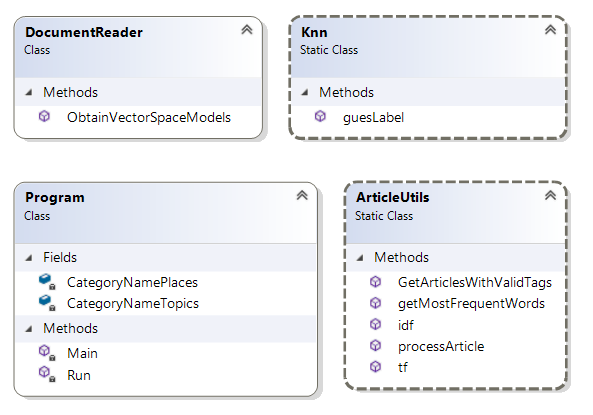
\includegraphics[width=1\textwidth]{/uml1.png}
	\caption{Diagram UML wygenerowany dla klas ogólnych.}
\end{figure}

\item IMetric - interfejs dla metryk, klasy implementujące owy interfejs:
\begin{itemize}
\item ChebyshewMetric -  klasa odpowiedzialna za metrykę Czebyszewa
\item ManhatattanMetric -  klasa odpowiedzialna za metrykę uliczną
\item EuclideanMetric - klasa odpowiedzialna za metrykę euklidesową\\
\end{itemize}

\begin{figure}[H]
	\centering
	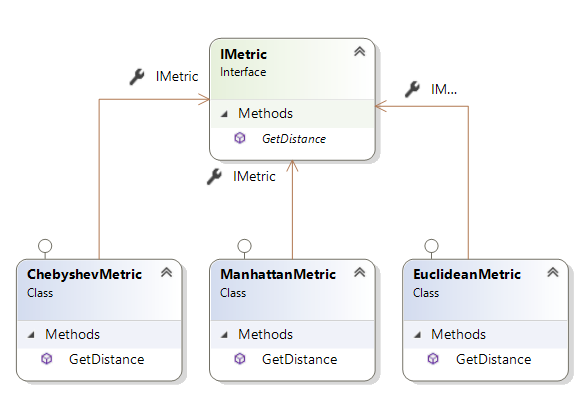
\includegraphics[width=1\textwidth]{/uml2.png}
	\caption{Diagram UML wygenerowany dla klas dotyczących metryk. }
\end{figure}

\item IStemmer - interfejs reprezentujący stemmer
\item Stemmer - reprezentacja stemera
\item EnglishStemer - stemer dla języka angielskiego

\begin{figure}[H]
	\centering
	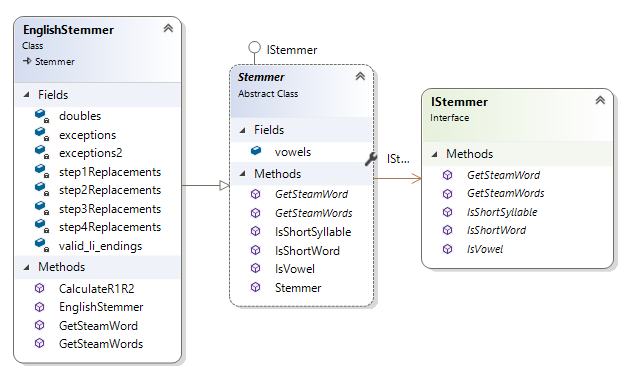
\includegraphics[width=1\textwidth]{/uml3.png}
	\caption{Diagram UML wygenerowany dla klas dotyczących procesu stemizacji.}
\end{figure}

\item Article - klasa reprezentująca pojedyńczy artykuł
\item ProcessedArticle - klasa dziecicząca po Article, reprezentuje przetworzony artykuł
\end{itemize}

\begin{figure}[H]
	\centering
	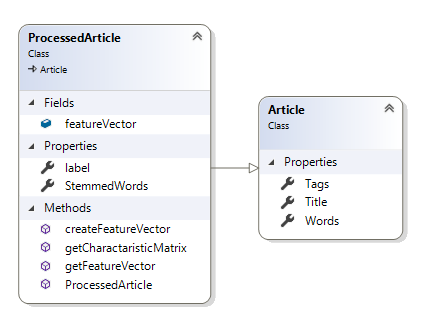
\includegraphics[width=1\textwidth]{/uml4.png}
	\caption{Diagram UML wygenerowany dla klas reprezentujących artykuły.}
\end{figure}

\section{Materiały i metody}
Klasyfikacja tekstów została wykonana wszystkimi dostępnymi metodami ekstrakcji cech dla wszystkich trzech metryk. Dla każdego przypadku testowego dokonano klasyfikacji tekstu dla k $\in$ \{2, 3, 5, 7, 10, 15, 20\} najbliższych sąsiadów. Wyniki porównano z faktyczną etykietą danego artykułu. \newline

Klasyfikacja dotycząca lokalizacji przeprowadzana była jedynie na danych, których pole places przyjmowało jedną z wartości: west-germany, usa, france, uk, canada, japan.
%Zbiór treningowy stanowił 60\% artykułów, zaś zbiór testowy 40\% artykułów.
\newline

Klasyfikacja dotycząca tematów przeprowadzana była jedynie na danych, które pole topics przyjmowało jedną z wartości: gold, cocoa, sugar, coffe, grain.
%Zbiory testowe stanowiły 60\% artykułów. \newline

%Danymi jakie sami przygotowaliśmy do analizy były teksty piosenek znanych artystów. Posiadały one jedną kategorię - author. Przyjmowało ono jedną z wartości: taylor swift, macklemore, twenty one pilots, eminem, ed sheeran, black eyed peas. Zbiór treningowy stanowił 60\% tekstów, zaś zbiór testowy 40\% tekstów.

Trzecim zestawem danych do analizy były nagłówki artykułów naukowych i cytaty o miłosci. Podzielone zostały przez tematykę - topic. Przyjmowało ono jedną z wartości: biology lub love.

\section{Wyniki}

{\color{blue}
W tej sekcji należy zaprezentować, dla każdego przeprowadzonego eksperymentu,
kompletny zestaw wyników w postaci tabel, wykresów itp. Powinny być one tak
ponazywane, aby było wiadomo, do czego się odnoszą. Wszystkie tabele i wykresy
należy oczywiście opisać (opisać co jest na osiach, w kolumnach itd.) stosując
się do przyjętych wcześniej oznaczeń. Nie należy tu komentować i interpretować
wyników, gdyż miejsce na to jest w kolejnej sekcji. Tu również dobrze jest
wprowadzić oznaczenia (tabel, wykresów) aby móc się do nich odwoływać
poniżej.}

\section{Dyskusja}
{\color{blue}
Sekcja ta powinna zawierać dokładną interpretację uzyskanych wyników
eksperymentów wraz ze szczegółowymi wnioskami z nich płynącymi. Najcenniejsze
są, rzecz jasna, wnioski o charakterze uniwersalnym, które mogą być istotne
przy innych, podobnych zadaniach. Należy również omówić i wyjaśnić wszystkie
napotakane problemy (jeśli takie były). Każdy wniosek powinien mieć poparcie
we wcześniej przeprowadzonych eksperymentach (odwołania do konkretnych
wyników). Jest to jedna z najważniejszych sekcji tego sprawozdania, gdyż
prezentuje poziom zrozumienia badanego problemu.}
\section{Wnioski}
{\color{blue}W tej, przedostatniej, sekcji należy zamieścić podsumowanie
najważniejszych wniosków z sekcji poprzedniej. Najlepiej jest je po prostu
wypunktować. Znów, tak jak poprzednio, najistotniejsze są wnioski o
charakterze uniwersalnym.}


\begin{thebibliography}{}
\bibitem{adam}
Methods for the linguistic summarization of data - aplications of fuzzy sets and their extensions, Adam Niewiadomski, Akademicka Oficyna Wydawnicza EXIT, Warszawa 2008
\end{thebibliography}
\end{document}
